\section{Termination of stabilization processes}\label{section: termination}
An \textbf{absorbing Markov chain} is a (not necessarily finite) Markov chain 
where each vertex has a path of finite length to an absorbing state.
For example, the infinite Markov chain 
shown in \cref{fig:rem unbounded hunger harmonic}
is absorbing, as a walker at any vertex $v_{i,j}$ can move 
to absorbing vertex $v_{0,0}$ within 2 moves.
We claim that in a finite absorbing Markov chain, 
the chip addition process at any vertex $v$ in the corresponding graph $G$ 
is guaranteed to terminate, regardless of the initial hunger state, 
and thus the chip addition operators $E_i$ are well-defined
for finite absorbing Markov chains.
This follows immediately
from the finiteness of $G$ and the following lemma:

\begin{lemma}\label{lemma: finite terminate}
For a finite absorbing Markov chain, each vertex $v$ gets visited
only finitely often in the hunger game
before the chip reaches an absorbing vertex.
\end{lemma}

\begin{proof}
The assumption that the Markov chain is absorbing
guarantees that for each $v$
there is a finite path $w_0,w_1,\dots,w_m$ 
such that $w_0$ is $v$, $w_m$ is an absorbing vertex,
and the transition probability from $w_i$ to $w_{i+1}$
is positive for all $0 \leq i \leq m-1$.
We prove the claim by induction on $m$.
The case $m=0$ is trivial,
as once the chip visits an absorbing vertex it is removed.
For a less trivial case, consider $m=1$.
For sake of contradiction, suppose $v=w_0$ is visited infinitely often.
Each time $w_0$ is visited, the hunger of $w_1$ increases by a fixed amount.
As $w_1$ is an absorbing vertex, we cannot visit it, as otherwise we would only visit $w_0$ finitely often before reaching an absorbing vertex.
This implies the hunger of $w_1$ increases unboundedly due to $w_0$ being visited infinitely often, contradicting the existence of an upper bound on hunger demonstrated in \cref{lemma: hunger bounded}.
Hence $w_0$ is visited finitely often, proving the case $m=1$.

The inductive step follows similar reasoning to the $m=1$ argument.
Suppose now that the claim is true for $m-1$,
so that $w_1$ is visited only finitely often.
Assume for sake of contradiction that $w_0$ is visited infinitely often, 
where each visit increases the hunger of $w_1$ by a fixed amount.
After $w_1$ is visited for the last time,
its hunger must grow without bound due to $w_0$
being visited infinitely often;
this contradicts \cref{lemma: hunger bounded}\,.
Hence the claim holds for all vertices.
\end{proof}

Since $G$ has only finitely many vertices,
each of which can fire only finitely many times before the chip is absorbed,
the chip must eventually be absorbed, as claimed.

A weakened version of this lemma applies to countable absorbing Markov chains.

\begin{proposition}\label{proposition: countable terminate}
On a countable absorbing Markov chain, if we add a chip
and then perform repeated firing, then either the chip eventually gets absorbed
or the chip is not confined within any finite subset of the state space.
\end{proposition}
\begin{proof}
If the Markov chain is finite, the result immediately follows 
from \cref{lemma: finite terminate}\,,
so assume the state space is countably infinite.
Suppose there is a finite subset $U$ of the state space $V$
such that the chip is always in $U$.
Consider the set $S$ given by
\begin{align*}
    S = U \cup \{ v \in V \mid \exists\, i\in U : P_{ij}>0\}.
\end{align*}
Because $U$ is finite and each vertex has finitely many outgoing edges, 
$S$ is also finite.
Crucially, as the chip is bounded within $U$, 
the only states whose hunger can change during the chip addition process 
are the states in $S$.
Hence, we may equivalently view the hunger game as acting upon 
the induced subgraph of $G$ formed from using $S$ as the vertex set, 
and from \cref{lemma: finite terminate} the result follows.
\end{proof}

\begin{remark}\label{remark: non-terminating infinite chip addition}
For infinite absorbing Markov chains,
it is possible for the chip to wander off
without being confined to any finite subset of the state space.
As a simple example, based on the goldbug system 
introduced by the second author of this article
as described in Kleber \cite{kleber2005goldbug}, 
take $\N\cup\{-1\}$ as the state space 
where states $-1$ and 0 are absorbing, and for $i \geq 1$, 
a walker at vertex $i$ 
moves to vertex $i-2$ and $i+1$ each with probability $\frac{1}{2}$, 
as shown in \cref{fig: goldbug system}\,.
Using the hunger state $\h$ where $\h_{-1} = \h_0 = \h_1 = -\frac{1}{2}$ 
and $\h_i = 0$ for $i > 1$, as shown in \cref{subfig: goldbug init}\,,
a chip inserted at state 1, as shown in \cref{subfig: goldbug insert}\,,
will move rightwards one state at a time to infinity;
the first few steps of the process 
are shown in \cref{subfig: goldbug fire 5}\,.
\begin{figure}[htbp]
    \centering
    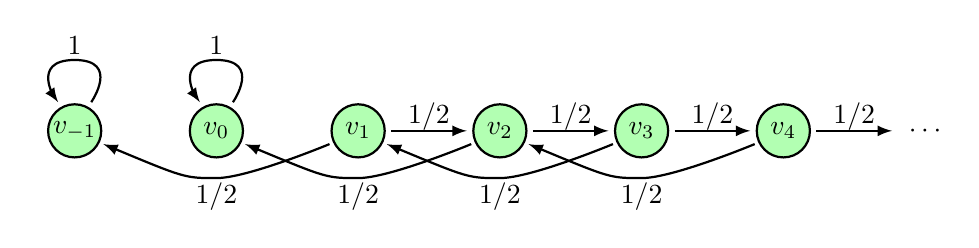
\begin{tikzpicture}[scale=0.6,font=\normalsize,baseline,thick]
        \foreach \x in {-1,...,4} {
            \filldraw[color=black,fill=green!30,thick] (3*\x + 3, 0) circle (16pt);
            \node at (3*\x + 3, 0) {$v_{\x}$};
        }
        \node at (3*6,0) {$\cdots$};
        % Self-loop absorbing
        \foreach \x in {0,...,1} {
            \draw [->,>=latex] plot [smooth,tension=5] coordinates {(3*\x+0.5*0.7,0.866*0.7) (3*\x+0,1.5) (3*\x-0.5*0.7,0.866*0.7)};
            \node at (3*\x,1.8) {1};
        }
        % Right edges
        \foreach \x in {2,...,5} {
            \draw[->,>=latex] (3*\x +0.7, 0) -- (3*\x + 3 -0.7, 0);
            \node at (3*\x +1.5,0.3) {1/2};
        }
        % Left edges
        \foreach \x in {2,...,5} {
            \draw [<-,>=latex] plot [smooth,tension=0.5] coordinates {(3*\x-2*3+0.866*0.7,-0.4*0.7) (3*\x-1*3,-1) (3*\x-0.866*0.7,-0.4*0.7)};
            \node at (3*\x-1*3,-1.4) {1/2};
        }
    \end{tikzpicture}
    \caption{The goldbug system.}
    \label{fig: goldbug system}
\end{figure}


\begin{figure}[htbp]
    \centering
    \begin{subfigure}{\textwidth}
    \centering
    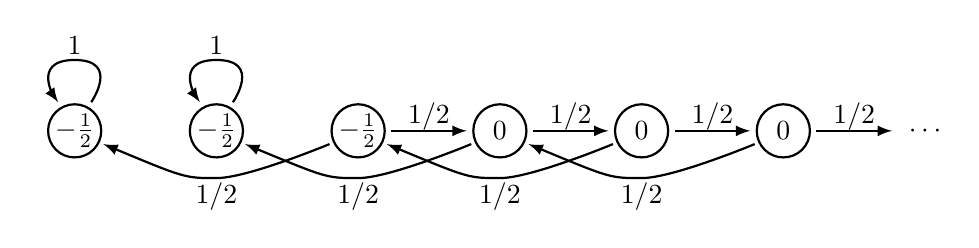
\begin{tikzpicture}[scale=0.6,font=\normalsize,baseline,thick]
        \foreach \x in {0,...,5} {
            \filldraw[color=black,fill=white,thick] (3*\x, 0) circle (16pt);
        }
        \foreach \x in {0,...,2} {
            \node at (3*\x,0) {$-\frac{1}{2}$};
        }
        \foreach \x in {3,...,5} {
            \node at (3*\x,0) {0};
        }
        \node at (3*6,0) {$\cdots$};
        % Self-loop absorbing
        \foreach \x in {0,...,1} {
            \draw [->,>=latex] plot [smooth,tension=5] coordinates {(3*\x+0.5*0.7,0.866*0.7) (3*\x+0,1.5) (3*\x-0.5*0.7,0.866*0.7)};
            \node at (3*\x,1.8) {1};
        }
        % Right edges
        \foreach \x in {2,...,5} {
            \draw[->,>=latex] (3*\x +0.7, 0) -- (3*\x + 3 -0.7, 0);
            \node at (3*\x +1.5,0.3) {1/2};
        }
        % Left edges
        \foreach \x in {2,...,5} {
            \draw [<-,>=latex] plot [smooth,tension=0.5] coordinates {(3*\x-2*3+0.866*0.7,-0.4*0.7) (3*\x-1*3,-1) (3*\x-0.866*0.7,-0.4*0.7)};
            \node at (3*\x-1*3,-1.4) {1/2};
        }
    \end{tikzpicture}
    \caption{The initial hunger state $\h$.}
    \label{subfig: goldbug init}
    \end{subfigure}
    \begin{subfigure}{\textwidth}
    \centering
    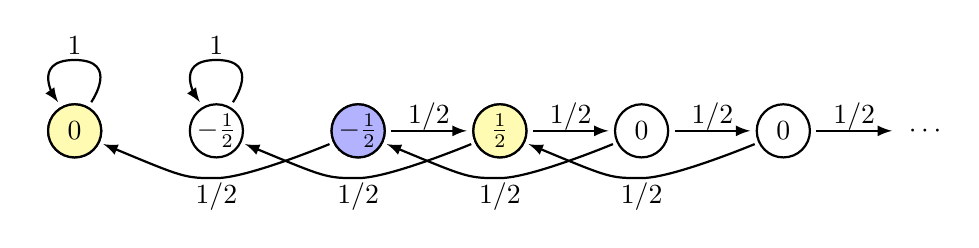
\begin{tikzpicture}[scale=0.6,font=\normalsize,baseline,thick]
        \foreach \x in {0,...,5} {
            \filldraw[color=black,fill=white,thick] (3*\x, 0) circle (16pt);
        }
        \filldraw[color=black,fill=blue!30,thick] (3*2,0) circle (16pt);
        \filldraw[color=black,fill=yellow!30,thick] (3*0,0) circle (16pt);
        \filldraw[color=black,fill=yellow!30,thick] (3*3,0) circle (16pt);
        \node at (3*0,0) {$0$};
        \node at (3*1,0) {$-\frac{1}{2}$};
        \node at (3*2,0) {$-\frac{1}{2}$};
        \node at (3*3,0) {$\frac{1}{2}$};
        \node at (3*4,0) {$0$};
        \node at (3*5,0) {$0$};
        \node at (3*6,0) {$\cdots$};
        % Self-loop absorbing
        \foreach \x in {0,...,1} {
            \draw [->,>=latex] plot [smooth,tension=5] coordinates {(3*\x+0.5*0.7,0.866*0.7) (3*\x+0,1.5) (3*\x-0.5*0.7,0.866*0.7)};
            \node at (3*\x,1.8) {1};
        }
        % Right edges
        \foreach \x in {2,...,5} {
            \draw[->,>=latex] (3*\x +0.7, 0) -- (3*\x + 3 -0.7, 0);
            \node at (3*\x +1.5,0.3) {1/2};
        }
        % Left edges
        \foreach \x in {2,...,5} {
            \draw [<-,>=latex] plot [smooth,tension=0.5] coordinates {(3*\x-2*3+0.866*0.7,-0.4*0.7) (3*\x-1*3,-1) (3*\x-0.866*0.7,-0.4*0.7)};
            \node at (3*\x-1*3,-1.4) {1/2};
        }
    \end{tikzpicture}
    \caption{$\h$ after inserting a chip at $v_1$, shown in blue. States with updated hungers are shown in yellow.}
    \label{subfig: goldbug insert}
    \end{subfigure}
    \begin{subfigure}{\textwidth}
    \centering
    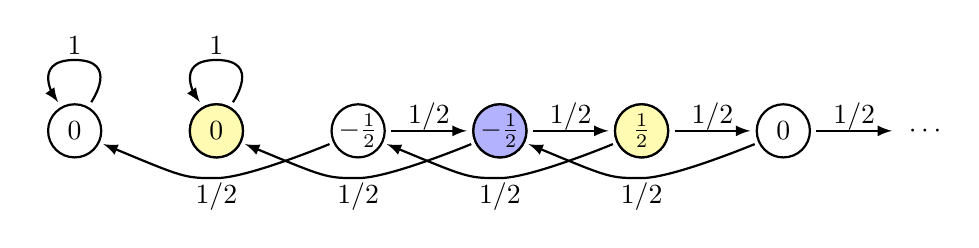
\begin{tikzpicture}[scale=0.6,font=\normalsize,baseline,thick]
        \foreach \x in {0,...,5} {
            \filldraw[color=black,fill=white,thick] (3*\x, 0) circle (16pt);
        }
        \filldraw[color=black,fill=blue!30,thick] (3*3,0) circle (16pt);
        \filldraw[color=black,fill=yellow!30,thick] (3*1,0) circle (16pt);
        \filldraw[color=black,fill=yellow!30,thick] (3*4,0) circle (16pt);
        \node at (3*0,0) {$0$};
        \node at (3*1,0) {$0$};
        \node at (3*2,0) {$-\frac{1}{2}$};
        \node at (3*3,0) {$-\frac{1}{2}$};
        \node at (3*4,0) {$\frac{1}{2}$};
        \node at (3*5,0) {$0$};
        \node at (3*6,0) {$\cdots$};
        % Self-loop absorbing
        \foreach \x in {0,...,1} {
            \draw [->,>=latex] plot [smooth,tension=5] coordinates {(3*\x+0.5*0.7,0.866*0.7) (3*\x+0,1.5) (3*\x-0.5*0.7,0.866*0.7)};
            \node at (3*\x,1.8) {1};
        }
        % Right edges
        \foreach \x in {2,...,5} {
            \draw[->,>=latex] (3*\x +0.7, 0) -- (3*\x + 3 -0.7, 0);
            \node at (3*\x +1.5,0.3) {1/2};
        }
        % Left edges
        \foreach \x in {2,...,5} {
            \draw [<-,>=latex] plot [smooth,tension=0.5] coordinates {(3*\x-2*3+0.866*0.7,-0.4*0.7) (3*\x-1*3,-1) (3*\x-0.866*0.7,-0.4*0.7)};
            \node at (3*\x-1*3,-1.4) {1/2};
        }
    \end{tikzpicture}
    % \caption{$\h$ after firing to $v_3$, shown in blue. States with updated hungers are shown in yellow.}
    % \label{subfig: goldbug fire 3}
    \end{subfigure}
    \begin{subfigure}{\textwidth}
    \centering
    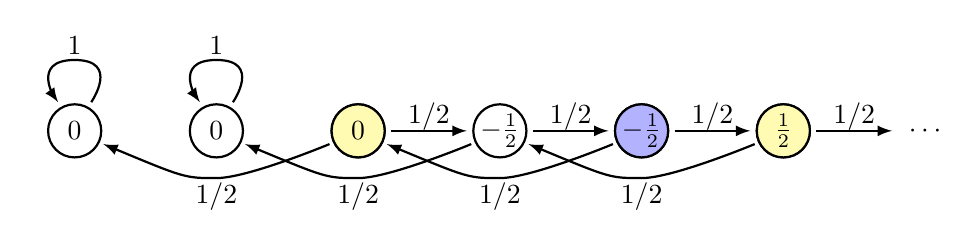
\begin{tikzpicture}[scale=0.6,font=\normalsize,baseline,thick]
        \foreach \x in {0,...,5} {
            \filldraw[color=black,fill=white,thick] (3*\x, 0) circle (16pt);
        }
        \filldraw[color=black,fill=blue!30,thick] (3*4,0) circle (16pt);
        \filldraw[color=black,fill=yellow!30,thick] (3*2,0) circle (16pt);
        \filldraw[color=black,fill=yellow!30,thick] (3*5,0) circle (16pt);
        \node at (3*0,0) {$0$};
        \node at (3*1,0) {$0$};
        \node at (3*2,0) {$0$};
        \node at (3*3,0) {$-\frac{1}{2}$};
        \node at (3*4,0) {$-\frac{1}{2}$};
        \node at (3*5,0) {$\frac{1}{2}$};
        \node at (3*6,0) {$\cdots$};
        % Self-loop absorbing
        \foreach \x in {0,...,1} {
            \draw [->,>=latex] plot [smooth,tension=5] coordinates {(3*\x+0.5*0.7,0.866*0.7) (3*\x+0,1.5) (3*\x-0.5*0.7,0.866*0.7)};
            \node at (3*\x,1.8) {1};
        }
        % Right edges
        \foreach \x in {2,...,5} {
            \draw[->,>=latex] (3*\x +0.7, 0) -- (3*\x + 3 -0.7, 0);
            \node at (3*\x +1.5,0.3) {1/2};
        }
        % Left edges
        \foreach \x in {2,...,5} {
            \draw [<-,>=latex] plot [smooth,tension=0.5] coordinates {(3*\x-2*3+0.866*0.7,-0.4*0.7) (3*\x-1*3,-1) (3*\x-0.866*0.7,-0.4*0.7)};
            \node at (3*\x-1*3,-1.4) {1/2};
        }
    \end{tikzpicture}
    % \caption{$\h$ after firing to $v_4$, shown in blue. States with updated hungers are shown in yellow.}
    % \label{subfig: goldbug fire 4}
    \end{subfigure}
    \begin{subfigure}{\textwidth}
    \centering
    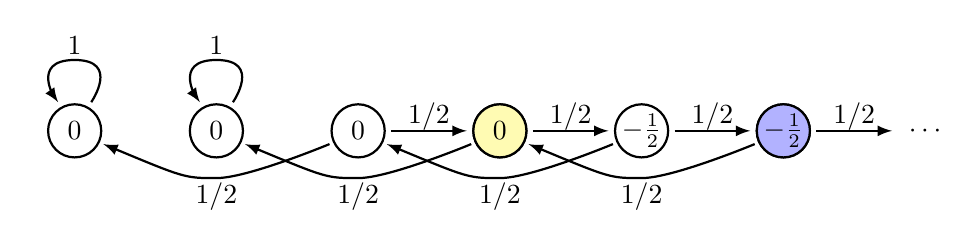
\begin{tikzpicture}[scale=0.6,font=\normalsize,baseline,thick]
        \foreach \x in {0,...,5} {
            \filldraw[color=black,fill=white,thick] (3*\x, 0) circle (16pt);
        }
        \filldraw[color=black,fill=blue!30,thick] (3*5,0) circle (16pt);
        \filldraw[color=black,fill=yellow!30,thick] (3*3,0) circle (16pt);
        \node at (3*0,0) {$0$};
        \node at (3*1,0) {$0$};
        \node at (3*2,0) {$0$};
        \node at (3*3,0) {$0$};
        \node at (3*4,0) {$-\frac{1}{2}$};
        \node at (3*5,0) {$-\frac{1}{2}$};
        \node at (3*6,0) {$\cdots$};
        % Self-loop absorbing
        \foreach \x in {0,...,1} {
            \draw [->,>=latex] plot [smooth,tension=5] coordinates {(3*\x+0.5*0.7,0.866*0.7) (3*\x+0,1.5) (3*\x-0.5*0.7,0.866*0.7)};
            \node at (3*\x,1.8) {1};
        }
        % Right edges
        \foreach \x in {2,...,5} {
            \draw[->,>=latex] (3*\x +0.7, 0) -- (3*\x + 3 -0.7, 0);
            \node at (3*\x +1.5,0.3) {1/2};
        }
        % Left edges
        \foreach \x in {2,...,5} {
            \draw [<-,>=latex] plot [smooth,tension=0.5] coordinates {(3*\x-2*3+0.866*0.7,-0.4*0.7) (3*\x-1*3,-1) (3*\x-0.866*0.7,-0.4*0.7)};
            \node at (3*\x-1*3,-1.4) {1/2};
        }
    \end{tikzpicture}
    \caption{$\h$ as the chip fires successively to $v_2$, $v_3$, and $v_4$, shown in blue. Updated hungers are shown in yellow.}
    \label{subfig: goldbug fire 5}
    \end{subfigure}
    \caption{A hunger state on the goldbug system where a chip inserted at $v_1$ goes to infinity.}
    \label{fig:rem non-terminating goldbug}
\end{figure}
\end{remark}

